\chapter{Introduction} \label{c:intro}

% xxx should I prevent citations from splitting across lines? Meaning
% the space before \cite{xxx} should be non-breaking?

%% RFI HSHQDC-14-00015
%% commercially available standoff - Brijot Gen 2, SET CounterBomber
%% TSA 700 AIT (advanced imaging technology) systems at 160 airports

For over thirty years the millimeter and submillimeter-wavelength spectrum has been the subject of intense interest for military and security imaging applications.
The reason for this interest is that the spectral region from \SIrange{100}{1000}{\GHz} offers a good compromise between transmission through obscuring materials (favoring lower frequencies) and spatial resolution (favoring higher frequencies) \cite{kruse_why_1981}.
``Obscuring'' here could refer to dust or fog for, e.g., helicopter landing assist systems, or clothing for concealed weapons detection.
This interest has helped to drive technological advances in sources, detectors, and other technologies at these wavelengths \cite{popovic_thz_2011,rogalski_terahertz_2011,rieke_detection_2003}.
This advancement has taken place in both ``active'' imaging, in which an observation target is illuminated by light and the reflections from that target are detected, and ``passive'' imaging, in which the target's thermal emissions are detected.

The millimeter and submillimeter astronomical community has also been interested in these wavelengths.
In particular, the desire to make more and more detailed maps of the Cosmic Microwave Background (\CMB) radiation has motivated this community to build instruments capable of higher and higher sensitivities.
During the 1980's and early 1990's individual cooled bolometric detectors capable of achieving photon-noise-limited performance were developed.
By 1994 it was clear that for astronomical applications the only way to increase sensitivity was to develop arrays of detectors, but at that time no technology for the production of monolithic arrays was yet available \cite{richards_bolometers_1994}.

The development of voltage-biased superconducting Transition Edge Sensor (\TES) detectors enabled the development of large-scale cryogenic detector arrays \cite{irwin_application_1995}.
These detectors are based on the use of thin superconducting films as the bolometer's thermometer element, and can be fabricated at large scale using standard lithographic techniques.
The basics of their operation and their advantages for passive imaging are described in \sectionref{sec:ch2-tes-basics} and \sectionref{sec:ch2-tes-passive}.
\chapterref{c:tes} provides more details on their behavior and operation.
To read out these detector arrays, several groups have developed Superconducting Quantum Interference Device (\SQUID) based multiplexed readout systems.
The last few decades have also seen advances in the development of mechanical cryocoolers capable of reaching liquid-helium temperatures, removing the need to transport liquid cryogens to the often remote locations that are used for ground-based millimeter and submillimeter astronomy.
This entire suite of technology~---~\TES\ detectors, multiplexed \SQUID\ readout, and cryogenics~---~is now mature and is routinely deployed on both ground and balloon-borne experiments in arrays containing up to 10,000 detectors \cite{holland_scuba-2:_2013}.

The development of this technology offers new opportunities for passive imaging for security and other applications.
Specifically, it is now possible to develop focal planes capable of video-rate imaging with temperature resolution of \SI{100}{\mK} or below.
This thesis describes the design and development of the National Institute of Standards and Technology (\NIST) \Imager, a system developed to detect concealed weapons at distances of \SIrange{16}{28}{\m} by producing video-rate images at \SI{350}{\GHz}.

An outline of this thesis is as follows.
This chapter provides an overview of passive millimeter and submillimeter wavelength imaging for security applications, and describes the reasons for using detectors operating at cryogenic temperatures.
\chapterref{c:specs} describes the specifications of the \Imager\ and gives an overview of the approach used to meet those specifications, as well as a brief summary of other passive imaging systems that use cryogenic detectors.
\chapterref{c:tes} presents the \TES\ theory required to understand this thesis.
The overall design of the system is described in \chapterref{c:sys-design} and the design of the detectors and focal plane is covered in \chapterref{c:det-design}.
\chapterref{c:det-array} describes measurements taken to characterize the first of four planned 251-detector sub-arrays.
The goal of this project is to generate video images at \SI{350}{\GHz}, and \chapterref{c:imaging} describes how the \Imager\ is used to do this, including quantitative evaluation of image quality.
\chapterref{c:summary} provides a brief summary of the achievements of this project and gives directions for future work.

The system described in this thesis is the result of work done by a number of different people both at \NIST\ and at other institutions.
The project was started by William Duncan, who also designed, procured, and assembled the optics.
Bob Schwall designed the cryogenic system.
The author of this thesis was responsible for commissioning the cryogenic system, designing the feedhorns used to guide light onto the detectors, the design of both the prototype and production detectors (including optical coupling components), layout of the detectors and all focal plane wiring, design and assembly of the focal plane, characterization of both the prototype detectors and first production detector sub-array, and optical testing of the system including the generation of video images.
Hsiao-Mei (Sherry) Cho fabricated the detectors.
The acknowledgments at the end of \chapterref{c:sys-design} and \chapterref{c:det-design} highlight particularly important contributions from other people both at \NIST\ and elsewhere.




\section{Security Imaging}

The frequency range \SIrange{100}{1000}{\GHz} is attractive for detection of concealed weapons or contraband because common clothing materials have high transmission in this range \cite{bjarnason_millimeter-wave_2004}.
As shown in \figref{fig:ch1-clothes-atmos-trans}, transmission through clothing steadily decreases as frequency increases.
This trend tends to push systems toward lower frequencies.
An example likely familiar to readers is the L3 ProVision systems operating at airport screening areas within the USA.
These are ``holographic radar'' systems operating at ~\SI{30}{\GHz}, intended for close-range portal screening, and are based on technology developed at the Pacific Northwest National Lab (PNNL) \cite{sheen_cylindrical_1998,mcmakin_dual-surface_2009}.
For applications in which it is acceptable to require individuals to pass through and pause at a particular location, these systems have excellent image quality.
Although the ProVision system takes still images with \abt{\SI{2}{s}} image acquisition time, similar portal screening systems with video-rate capabilities are also under development \cite{lyons_reflect-array_2013}.

\begin{figure*}
\centering
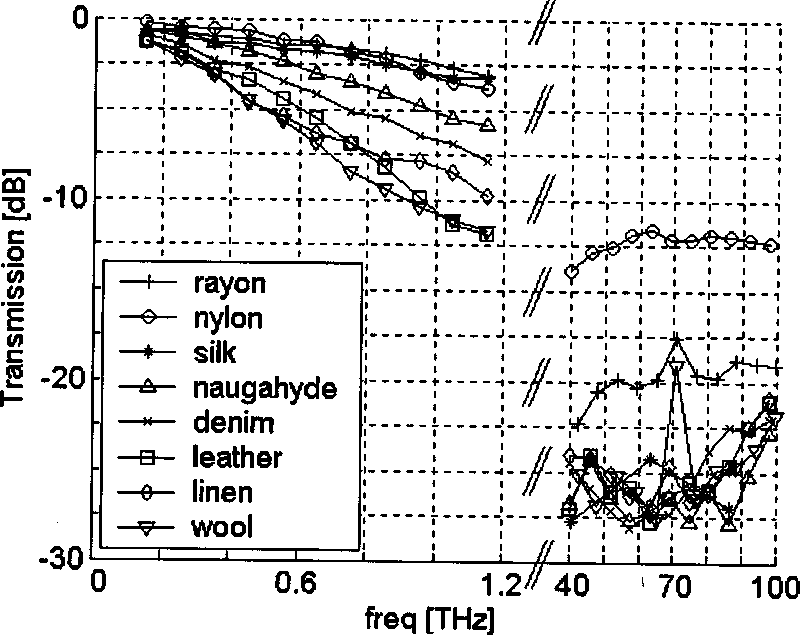
\includegraphics{drawings/ch1-clothes-bjarnason.pdf} \\
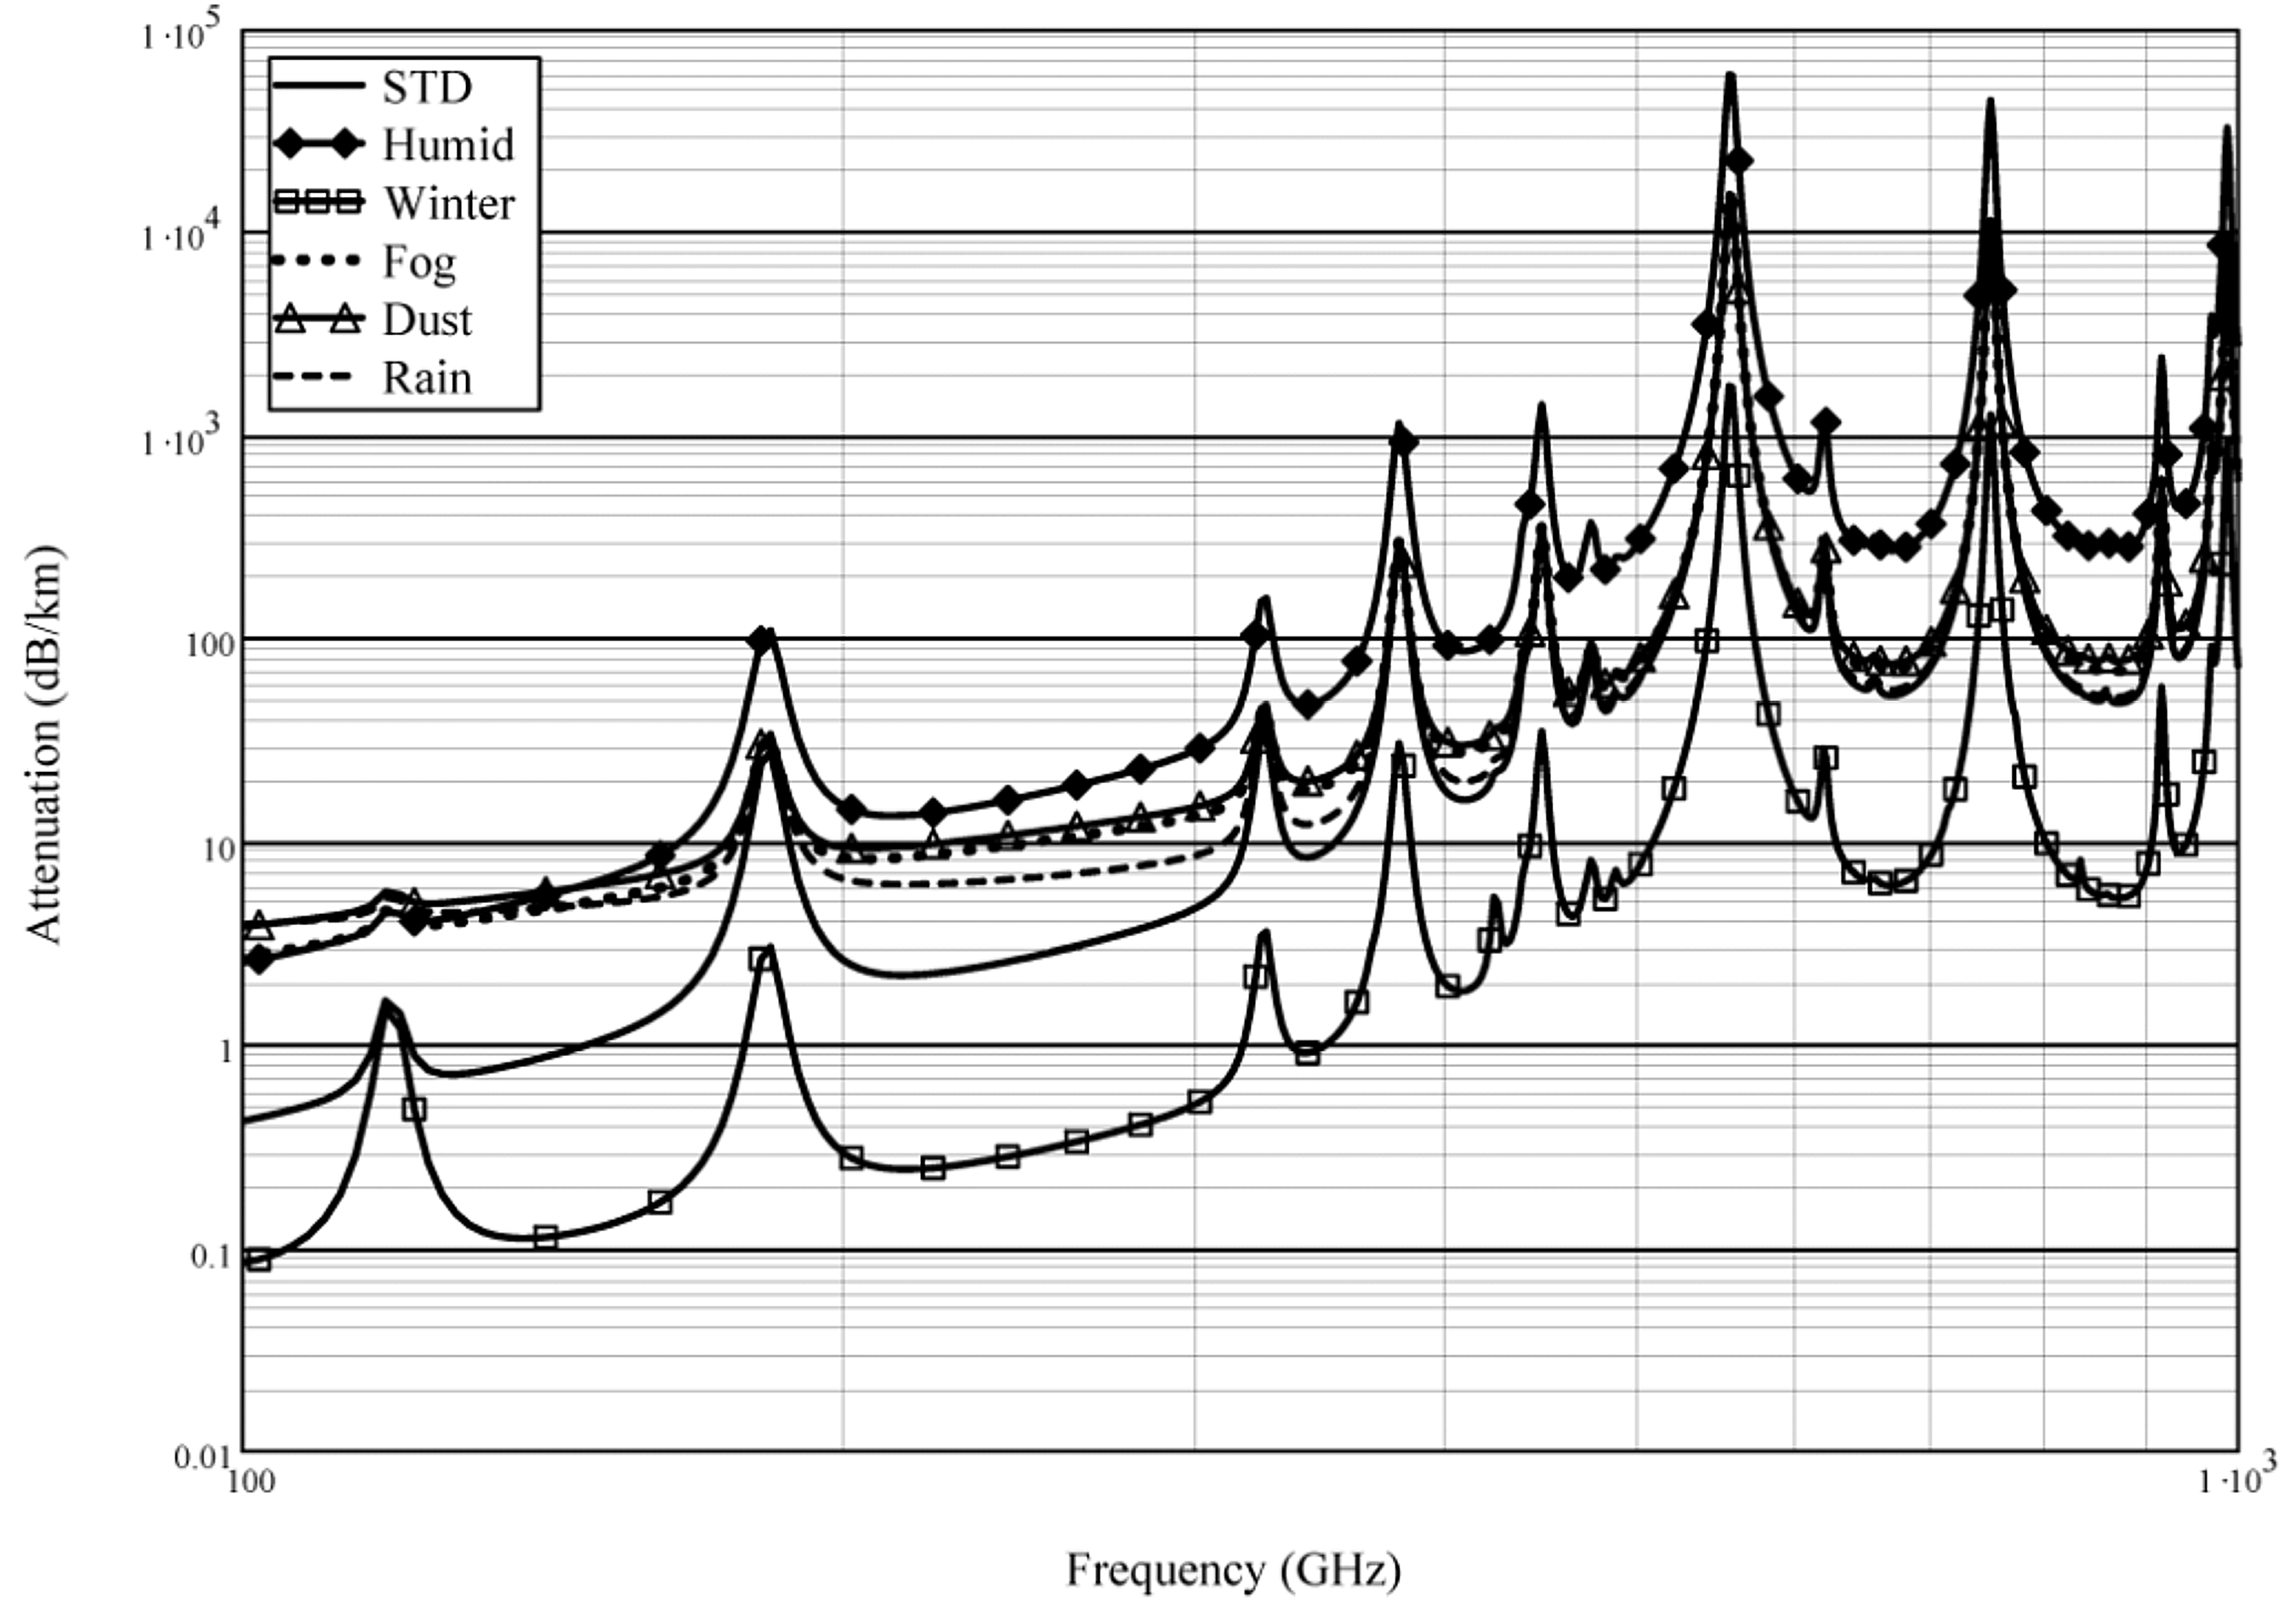
\includegraphics{drawings/ch1-atmos-trans.pdf}
\caption[Clothing and Atmospheric Transmission vs Frequency]{
  \textbf{Left}
  Plot of clothing transmission vs frequency.
  Taken from \cite{bjarnason_millimeter-wave_2004}.
  As frequency increases, transmission through all kinds of clothing decreases.
  The \SI{-10}{\dB} observation band of the \Imager\ is highlighted (\SIrange{318}{376}{\GHz}).
  \textbf{Right}
  Plot showing attenuation through the atmosphere at sea level pressure for different weather and particulate conditions.
  Under the worst conditions in the \Imager's band, attenuation would be \abt{\SI{1.2}{\dB}} over \SI{16}{\m}, and a factor of five better under standard conditions.
  At the \SI{640}{\GHz} band, attenuation under standard conditions is the same as the worst conditions at \SI{350}{\GHz}, and a factor of 6 worse again under the worst conditions.
  Taken from \cite{appleby_standoff_2007}.
}
\label{fig:ch1-clothes-atmos-trans}
\end{figure*}

But there are other applications and operational scenarios in which portal screening systems are not feasible.
One example is detection of suicide bomb belts, a scenario in which is it desirable to make a detection while the person being observed is some distance away.
In these scenarios it is not always reasonable to expect observation targets to be stationary, so video-rate imaging is also required.
These applications are generally referred to as ``standoff'' detection because the imaging system ``stands off'' some distance from the target being imaged.

For these applications the choice of optical frequency is less clear than for portal imaging, because an additional factor to consider is spatial resolution of the resulting images.
The lower frequencies favored by clothing transmission also imply worse spatial resolution for a fixed optical aperture size.
The angular resolution $\theta$ achievable by an aperture of diameter $D$ observing at wavelength $\lambda$ is, by the Raleigh criterion \cite{born_principles_1999},
\begin{equation} \label{eqn:ch1-raleigh}
  \theta \sim 1.2 \lambda / D.
\end{equation}
For portal screening this is not prohibitive; the L3 Provision system has an effective aperture of \SI{1.7}{\m} \cite{mcmakin_dual-surface_2009}.
But for standoff distances of \SI{10}{\m} or more, a system operating at \SI{30}{\GHz} would need an aperture of size \abt{\SI{8}{\m}} in order to achieve \SI{1}{\cm} resolution.
This strongly drives the choice of frequency for standoff detection to frequencies above \SI{100}{\GHz}.

A final factor to consider in the choice of operating frequency is atmospheric transmission.
As shown in \figref{fig:ch1-clothes-atmos-trans}, not only does transmission through clothing fall with increasing frequency, but transmission through the atmosphere does as well, although the trend is not monotonic.
For the \SI{350}{\GHz} band used by the \Imager, under the worst atmospheric conditions (hot and humid weather) transmission over \SI{16}{\m} is \abt{\SI{75}{\percent}}.
Indoors, in the dry winter climate of Boulder, CO transmission over \SI{16}{\m} will be close to \SI{100}{\percent}.

Security imaging systems for standoff applications broadly fall into two categories: ``active'' and ``passive'' \cite{appleby_standoff_2007,appleby_passive_2004}.
Active systems illuminate the target to be imaged with light and use the reflected light to obtain an image.
Passive systems detect thermal blackbody emissions that are naturally emitted by all objects.
Because the temperatures of objects being viewed are so low (\abt{\SI{300}{\K}}), active systems would seem to have an inherent signal-to-noise advantage over passive systems.
But active imaging suffers from two problems that to-date have allowed passive imaging systems to generally exceed the image quality achieved with active systems.

\subsection{Active Standoff Imaging}

Both problems stem from the fact that active imaging systems generally use single-moded coherent sources of light; see \cite{petkie_active_2008} for a good overview of the issues.
The first problem is generally referred to as ``specular reflections''.
This refers to the fact that the intensity of light that is reflected off of the target and subsequently detected by the active imaging system is strongly dependent on the angle of the target relative to the illuminating beam.
This leads to strong highlight areas in active images which can be \SI{40}{\dB} or more higher than neighboring areas, making images difficult to interpret.
For a concrete example, the reader can imagine the way that sunlight at just the right angle can reflect off of the fender of another car on the road, making it difficult for their eyes to interpret what they are looking at.
This problem would be even worse if the Sun's illumination were single-moded rather than multi-moded.

The second problem is known as ``speckle''.
When a coherent light source is diffusely reflected from a surface which varies on distance scales comparable to or larger than a wavelength, some areas of the surface will randomly be oriented more favorably than others for reflecting light back to the system.
This leads to a random distribution of bright spots in the image known as speckle \cite{goodman_fundamental_1976}.
This phenomena acts as a kind of noise in active images, and the signal-to-noise ratio of active imaging systems is often limited by speckle rather than noise inherent in the detection system itself.

The active imaging community has long been aware of these issues and is working to address them.
One recent approach uses modulated multi-moded illumination to avoid these issues \cite{petkie_multimode_2012,patrick_elimination_2012}.
Another approach is to use active illumination to build a radar system.
Because the radar system detects phase differences rather than intensity differences, it should be less susceptible to specular reflections and speckle.

The active imaging system that at this time is closest to producing video-rate imaging largely free of specular-reflection and speckle artifacts is the \SI{340}{\GHz} radar system developed at the Jet Propulsion Laboratory \cite{cooper_thz_2011}.
This system operates at standoff distances of \SI{16}{\m} achieving a spatial resolution of \SI{1}{\cm} at 4 frames per second.

% xxx can I bring in the idea that passive imaging allows covert surveillance

\section{Required Image Noise for Passive Imaging} \label{sec:ch1-netd-reqs}

Passive imaging does not suffer from the problems of specular reflection and speckle.
Instead, the primary challenge for passive imaging is implementing sufficiently sensitive detectors to achieve low-noise images at video frame rates.
One commonly used figure-of-merit for noise in a passive imaging system is the Noise Equivalent Temperature Difference (\NETD) of the image, defined as the difference in the temperature distribution at the observation target which can not be distinguished from noise in the image.
Few detailed studies of the \NETD\ required for detection of concealed weapons or other contraband have been published, but the ``lore'' of the field is that for non-metallic concealed threats in an indoor environment, image signals are \SIrange{0.5}{1.0}{\K}, with \SI{200}{\mK} or lower \NETD\ required for detection.
One published estimate gives \SI{100}{\mK} as the required noise level \cite{salmon_scene_2004} under some scenarios.
The remainder of this section justifies this lore quantitatively.

To estimate the required \NETD\ for a passive imaging system we must investigate both the required signal-to-noise for detection and the expected contrast (signal) in passive imaging scenarios.
The required signal-to-noise ratio for object detection depends on the size of the object \cite{steven_w._smith_scientist_1997}.
This is explored in a simple way in \figref{fig:ch1-sn}.
This figure shows a sequence of simulated images with a \SI{22.5}{\cm} (\SI{9}{in}) knife in the middle left of the image, and a $2\times2$ bright pixel block in the upper right.
At a signal to noise ratio of 1, the knife is barely visible if you know where to look for it.
At a signal-to-noise ratio of 2 the knife becomes visible but the much smaller block is not.
The block can barely be made out at \SN\ 4, and at \SN\ 6 both block and knife are clearly visible.
Based on this I assume a required \SN\  of 4 for detection; this means that in order to reliably detect an object with contrast \SI{1}{\K} in an image, the required \NETD\ is \SI{0.25}{\K}.

\begin{figure*}
\centering
\includegraphics{drawings/ch1-sn.pdf}
\caption[Signal-to-noise ratio for object detection]{
  Exploration of signal-to-noise ratio (\SN) required for object detection.
  Each simulated image contains $100 \times 100$ pixels.
  In the middle left of each image is a simple \SI{22.5}{\cm} model of a knife.
  In the upper right a $2\times2$ block of pixels has been set to be bright.
  Gaussian noise was added to each image with a level appropriate for the \SN\ listed in the title.
  At $\SN\ = 1$ the knife is perhaps visible if you know where to look but the block is not.
  At $\SN\ = 2$ the knife become visible but the much smaller block is not.
  The block begins to become visible at $\SN\ = 4$, and is clearly visible at $\SN\ = 6$.
}
\label{fig:ch1-sn}
\end{figure*}

The contrast in a passive image is set by the temperatures, emissivities and transmittivities of the objects being imaged, along with the temperature of the ambient light.
Although passive imaging systems detect optical power, not the temperature of objects directly, these systems operate in the Raleigh-Jeans limit where the optical power per mode is directly proportional to temperature; see \sectionref{sec:ch1-passive-tech}.
\figref{fig:ch1-t-tot} depicts the situation schematically.
We consider an object at temperature $T_{1}$ with emissivity $\epsilon_1$, covered by an object at temperature $T_{cov}$ and transmittivity $\tau_{cov}$.
The entire scene is illuminated by blackbody radiation at temperature $T_{amb}$.
We assume that the covering object has no reflection, so that $\epsilon_{cov} = 1 - \tau_{cov}$.
The total temperature seen by an observer looking at the object through the covering will be
\begin{equation} \label{eqn:ch1-t-tot}
  T_{tot,1} = (1 - \epsilon_{1}) \tau_{cov}^2 T_{amb} + 
           (1 + \tau_{cov}(1 - \epsilon_{1}))(1-\tau_{cov}) T_{cov} + 
           \tau_{cov} \epsilon_{1} T_1
\end{equation}
A second object behind the cover with temperature $T_2$ and emissivity $\epsilon_2$ will appear to have a temperature given by \eqnref{eqn:ch1-t-tot} with the subscript 1 replaced by 2 everywhere.
The contrast seen between these two objects will then be
\begin{equation} \label{eqn:ch1-delta-t}
  \Delta T_{1,2} = \tau_{cov} \left[ (\epsilon_2 - \epsilon_1) \tau_{cov} T_{amb} + 
                                    (\epsilon_2 - \epsilon_1) (1-\tau_{cov}) T_{cov} + 
                                    (T_1 \epsilon_1 - T_2 \epsilon_2) \right]
\end{equation}
This equation shows that in order for contrast to appear in the image, we require a difference in temperature or emissivity between the two objects, or both.

\begin{figure*}
\centering
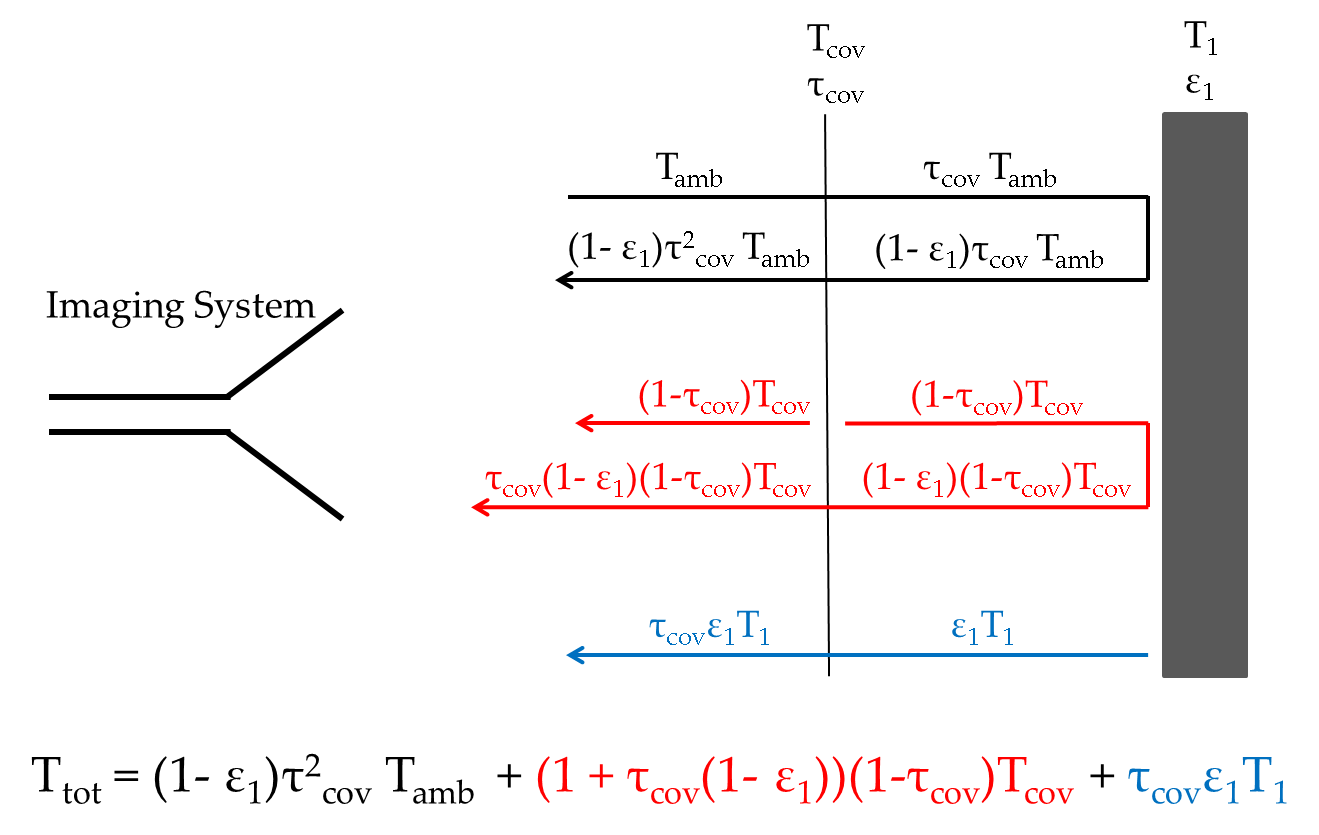
\includegraphics[width=6in]{images/ch1-t-tot.png}
\caption[Apparent temperature of a covered illuminated object]{
  Schematic showing total temperature seen looking at an object at temperature $T_1$ with emissivity $\epsilon_1$ through a cover at temperature $T_{cov}$ with transmittivity $\tau_{cov}$, all illuminated by ambient temperature $T_{amb}$.
  The Raleigh-Jeans limit is assumed to hold, so that emitted optical power is directly proportional to the temperatures of the emitting sources.
  The object is assumed to have no transmission and the cover to have no reflection.
  The black arrows indicate transmission of ambient light through the cover, reflecting off the object, and passing back through the cover to the detecting system.
  The red arrows show the emission of the cover, which reaches the detector both directly and after reflecting off the object.
  The blue arrows show the emission of the object itself.
}
\label{fig:ch1-t-tot}
\end{figure*}

We consider the case where the objects have the same temperature but different emissivities.
This would be the case for objects strapped next to skin, underneath clothing for a period of time so that objects come into thermal equilibrium with the body.
In this case \eqnref{eqn:ch1-delta-t} reduces to
\begin{equation}
  \Delta T_{1,2} = \tau_{cov} (\epsilon_1 - \epsilon_2) \left[ (1 - \tau_{cov}) (T - T_{cov}) + \tau_{cov} (T - T_{amb}) \right].
\end{equation}
In security screening scenarios we would typically expect $T > T_{cov} > T_{amb}$, so the rightmost factor will be positive.
If we further assume that $T_{cov}$ is midway between $T$ and $T_{amb}$, then this further simplifies to
\begin{equation} \label{eqn:ch1-delta-t-simple}
  \Delta T_{1,2} = \frac{1}{2}\tau_{cov}(1+\tau_{cov}) (\epsilon_1 - \epsilon_2) (T - T_{amb}).
\end{equation}
The factor of $\frac{1}{2}$ represents that fact that at low $\tau$, under these assumptions, the contrast is dominated by the difference in temperature between the cover and the object, which is half of the difference between the object and the ambient light.

Outdoors, $T_{amb}$ will have contributions both from the ground (or structures/vegetation at ground level) and from the sky.
The sky temperature depends strongly on the weather, and at \SI{350}{\GHz} could be as low as \SI{100}{\K} on a clear winter day, or approach \SI{310}{\K} on a hot day with high humidity \cite{appleby_standoff_2007}.
Depending on the temperature and emission properties of local ground cover, under the worst-case scenario $T_{amb}$ outdoors could be very close to human body temperature.
This means that requirements on \NETD\ for outdoor imaging in the worst-case scenarios could easily be \SI{200}{\mK} or lower, which motivates the search for imaging systems with \NETD\ at or below \SI{100}{\mK} for outdoor applications. 

Indoors, $T_{amb}$ will be determined by the temperature of the room, typically $\SI{295}{\K} = \SI{72}{\fahrenheit}$.
We can take as a challenging scenario the detection of plastic explosives hidden beneath a woolen sweater.
From \cite{bjarnason_millimeter-wave_2004} we use $\tau_{cov} = 0.5$ and from \cite{appleby_standoff_2007} we can take $\epsilon_{explosive} - \epsilon_{skin} = 0.08$, a case where the emissivity of the explosive is higher than that of skin.
\eqnref{eqn:ch1-delta-t-simple} gives $\Delta T_{1,2} = \SI{0.45}{\K}$, or a required \NETD\ of \SI{112.5}{\mK} assuming a required \SN\ of 4.
If the explosive material is cooler than body temperature then the requirements on \NETD\ will be eased, but it is the worst-case scenarios that should drive system requirements.

From this we conclude that \NETD\ values of \SI{100}{\mK} or lower are required for the most challenging passive imaging scenarios.
The above analysis represents a simplification of any real-world scenario.
But in the absence of any published studies of measured contrast in a variety of scenarios, we are justified in using these estimates as guidelines for the development of a system intended to perform those studies.
The question remains as to what technology is capable of reaching this level of sensitivity.

\section{Passive Imaging Technology} \label{sec:ch1-passive-tech}

One option for the detection of light at \SIrange{100}{1000}{\GHz} is the use of incoherent direct detectors, including photo-diodes and other photon detectors as well as bolometers.
These devices are square-law detectors, sensitive to the square of the incident electromagnetic field, i.e. to incident optical power.
They can be characterized by a Noise Equivalent Power (\NEP), defined as the detected signal power equal to the standard deviation of the detector noise in a \SI{1}{\Hz} post-detection bandwidth.
To convert the \NEP\ of the detectors to an \NETD\ for an image, we must first have a conversion between detected optical power and source temperature.
For a detector sensitive to $M$ spatial modes of the electromagnetic field and with total optical efficiency $\eta_{tot}$, the optical power detected per unit optical frequency is given by the Planck law in the form \cite{richards_bolometers_1994}
\begin{equation} \label{eqn:ch1-planck}
  P_{\nu}(\nu,T) d \nu = \eta_{tot} M h \nu \frac{1}{e^{\frac{h \nu}{k_B T}} - 1} d \nu,
\end{equation}
where $h$ is Planck's constant, $k_B$ is Boltzmann's constant, and $T$ is the temperature of the source.
For detection of light around \SI{350}{\GHz}, and source temperatures in the range \SIrange{50}{300}{\K}, the Raleigh-Jeans approximation
\begin{equation}
  \frac{1}{e^{\frac{h \nu}{k_B T}} - 1} \approx \frac{k_B T}{h \nu}
\end{equation}
holds to within \SI{20}{\percent}, so that the total optical power in an optical bandwidth reduces to 
\begin{equation}
  P_{\nu} = \eta_{tot} M k_B T \Delta \nu.
\end{equation}
This allows us to convert a detector \NEP\ to a Noise Equivalent Temperature (\NET) via
\begin{equation}
  NET = \frac{NEP}{\eta_{tot} M k_B \Delta \nu}.
\end{equation}

To convert this detector \NET\ to an \NETD\ for an image, we make the assumptions that noise for each detector can be modeled as an uncorrelated Gaussian noise source, so that the noise for a given pixel in the image will be given by the \NET\ divided by the square root of twice the integration time for that pixel across all detectors\footnote{%
  The factor of 2 accounts for the fact that \NEP\ is defined to give the total variance of a signal when integrated to only the Nyquist frequency, whereas the full bandwidth up to the sampling frequency is available for reducing noise.
}. 
We consider an image covering an area $A$ with square pixels of side length $s$, produced by an imaging system with $N$ detectors and video frame rate of $FPS$.
The integration time per pixel $\tau_{int}$ will then be given by
\begin{equation}
  \tau_{int} = \frac{N / FPS}{A / s^2},
\end{equation}
and so the \NETD\ of each image will be
\begin{align}
  NETD & = \frac{NET}{\sqrt{2\tau_{int}}} \\
       & = \frac{NET}{\sqrt{ 2 \frac{N / FPS}{A / s^2}}} \\
       & = \frac{NEP}{\eta_{tot} M k_B \Delta \nu} \frac{1}{s} \sqrt{\frac{A\,FPS}{2 N}} .
       \label{eqn:ch1-netd-defn}
\end{align}

Micro-bolometers have an advantage in that they can be fabricated in arrays with relative ease.
Typical \NEP\ values for uncooled micro-bolometers in the millimeter-wave region are \Pnoisep{10}--\Pnoisep{100} \cite{nemarich_microbolometer_2005,rogalski_terahertz_2011}.
In order to convert this \NEP\ into an \NETD\ we must make some assumptions.
In order to achieve sufficient spatial resolution, detectors at these wavelengths are typically sensitive to two modes, one per polarization, so we set $M = 2$.
We can generously assume a staring array with one detector per image pixel, so that $\sqrt{A/N}/s = 1$.
A very good optical efficiency would be $\eta_{tot} = 0.5$, and a typical bandwidth at \SI{350}{\GHz} is \SI{35}{\GHz}.
The minimum frame rate for video imaging is approximately 6 frames per second.
Plugging these numbers into \eqnref{eqn:ch1-netd-defn} leads to an \NETD\ of \SI{50}{\K} for the best-case scenario of \Pnoisep{10} \NEP.
This is more than two orders of magnitude higher than the requirements discussed in \sectionref{sec:ch1-netd-reqs}.

Perhaps the most promising approach for room-temperature direct detection of millimeter and submillimeter light is an approach using backward tunnel diodes for operation at \SI{90}{\GHz}, which has achieved \Pnoisep{0.1} \NEP\ with a 32-channel linear array \cite{schaffner_wideband_2008,wikner_demonstration_2009}.
Under the same assumptions as in the previous paragraph, a staring array would achieve \SI{5}{\K} \NETD, still insufficient to achieve the \NETD\ requirements of \sectionref{sec:ch1-netd-reqs}.

A second option for passive imaging is the use of coherent heterodyne detectors \cite{rieke_detection_2003,rogalski_terahertz_2011}.
This technology has advanced sufficiently that commercial systems are available today.
The most promising option to-date is the ThruVision\footnote{Digital Barriers plc, London, UK. \url{http://www.digitalbarriers.com/products/thruvision}} family of imagers operating at \SI{250}{\GHz} \cite{mann_first_2009,digital_barriers_extra_????}.
Video frame rates are 6 frames per second and claimed \NETD\ is \SI{1}{\K}.
The system also has the ability the average consecutive video frames when the target being observed is stationary, in order to reduce noise.
The system has standoff distances up to \SI{15}{\m}, but with poor spatial resolution due to apertures only \abt{\SI{20}{\cm}} in diameter.

The Microsemi GEN 2 system\footnote{%
Microsemi Corporation, Aliso Viejo, CA. This technology was acquired from Brijot systems in 2011.}
is another commercial system operating at \SI{90}{\GHz}.
This system achieves \SI{5}{\cm} resolution at 4--12 frames per second at standoff distances of a few meters.
\NETD\ is not quoted, but is presumably not better than \SI{1}{\K}.
The performance of these two room-temperature imaging systems is listed in \tableref{tab:ch2-sys-compare}, along with other cryogenic passive imaging systems and the \Imager\ described in this thesis.

The conclusion is that to achieve sufficient \NETD\ and spatial resolution for passive standoff imaging at distances of \SI{10}{\m} and greater, room temperature detectors to-date do not have sufficient noise performance.
For this reason the \Imager\ uses \TES\ bolometers operating at cryogenic temperatures.
The next chapter gives the specifications for our system and explains how \TES\ bolometer arrays meet those specifications.
